\section{Hardware}\label{ch:hardware}

\subsection{Wahl der Sensoren / Aktoren}

Zentraler Punkt unseres Projektes stellte auch die Entwicklung echter Sensorknoten dar, um auf reale Daten von Sensoren zurückgreifen bzw. verschiedene Aktoren ansteuern zu können. Hierbei wurden im ersten Schritt Sensoren und Aktoren gesucht, welche für unser Projekt in Frage kommen und anschließend nach Priorität geordnet, um die Abarbeitungsreihenfolge zu bestimmen.

Sensoren:
\begin{itemize}
\item BME280: Temperatur, Luftfeuchtigkeit, Luftdruck
\item HR-SR501: Anwesenheitserkennung/Bewegungsmelder
\item KY-037: Mikrofon/Schallpegel zur Bestimmung der Lautstärkenbelastung
\end{itemize}

Aktoren:
\begin{itemize}
\item LEDs (Rot – Gelb – Grün – Blau) als Statusanzeige
\item LCD-Display zur Anzeige verschiedener Informationen (4 Eingabetasten für mögliche Benutzereingabe)
\item Piezo-Buzzer zur Wiedergabe von Statustönen
\end{itemize}

\subsection{Konzeptionierung}

Bei der Entwicklung des Knotens wurde vor allem darauf geachtet, dass dieser eine generische Schnittstelle für die Sensoren/Aktoren bereitstellt, um diese zu einem späteren Zeitpunkt um weitere Senor-/Aktorelemente erweitern zu können. Hierfür wurden zunächst aus den gegebenen Elementen die benötigten Funktionen (Special Functions, kurz SF) extrahiert:

\begin{itemize}
\item Analog-Digital-Wandlung (z.B. MQ-135, KY-037)
\item Digital Lesen (z.B. Hr-SR501, LCD-Display Taster)
\item Digital Schreiben (z.B. LEDs, LCD-Display)
\item Frequenz-Modulation (Piezo-Buzzer)
\end{itemize}

Zudem wurde ein genormter Daten-Bus implementiert, welcher es ermöglicht, digitale Sensoren/Aktoren und Erweiterungsplatinen anbinden zu können. Hier kommt der I²C-Bus zum Einsatz, welcher eine synchrone Kommunikation über eine Zweidrahtleitung ermöglicht. Der Raspberry-Pi übernimmt dabei die Rolle des Masters, welcher die Kommunikation leitet. Die Adressierungsfunktionalität erlaubt es dabei bis zu 126 Slaves einzubinden. Auch der eingesetzte BME280 implementiert diese Schnittstelle und wird in unserem Projekt darüber angesteuert.

Bei der Analyse benötigten Funktionen stellte sich schnell heraus, dass die GPIO-Pins des Raspberry-Pi’s diese Anforderungen nicht erfüllen kann, da dieser beispielweise keine ADC-Funktionalität bereitstellt, sowie diverse Sensoren auf 5V Spannungslevel kommunizieren, während die IO’s es Raspberry-Pi’s nur 3,3V kompatibel sind. Deswegen wurde der I²C-Datenbus um einen Mikrocontroller erweitert. Dieser dient als Erweiterung der GPIOs des Pi’s, stellt die 5V Kompatibilität bereit, um die restlichen Anforderungen zu erfüllen. 

\begin{figure}[h!]
      \centering
      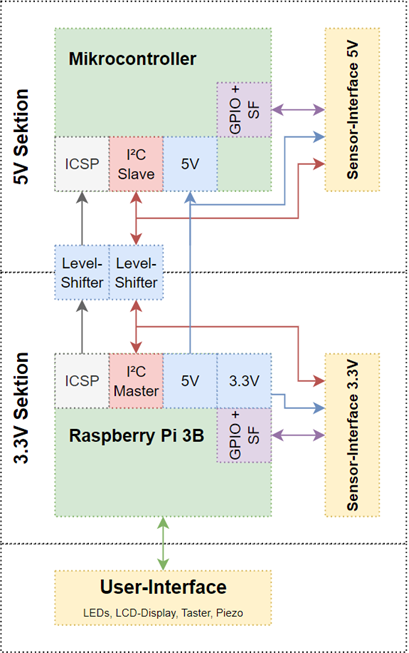
\includegraphics[scale=0.6]{abbildungen/schaltplan.png}
      \caption{Interne Verbindungen und Schnittstellen auf einem Sensorknoten}
 \end{figure}

 \subsection{Hardwareentwurf}

 Anschließend wurde ein Schaltplan mit den benötigten Komponenten entworfen und mit einem Steckbrettaufbau validiert. Für eine einheitliche und saubere Verkabelungslösung wurde anschließend eine Aufsteckplatine passend zu dem Raspberry Pi entworfen, welche alle notwendigen Hardware-Komponenten enthält. Ebenfalls wurden alle Userinterface-Elemente wie Display, Taster, Piezo-Buzzer uvm. mit aufgebracht, welche auf jeden Knoten vorhanden sind. Seitlich befinden sich das 3.3V und 5V Sensorinterface, ausgeführt als Stiftleiste, an welches dynamisch die Sensoren angeschlossen werden kann. 

 \begin{figure}[h!]
      \centering
      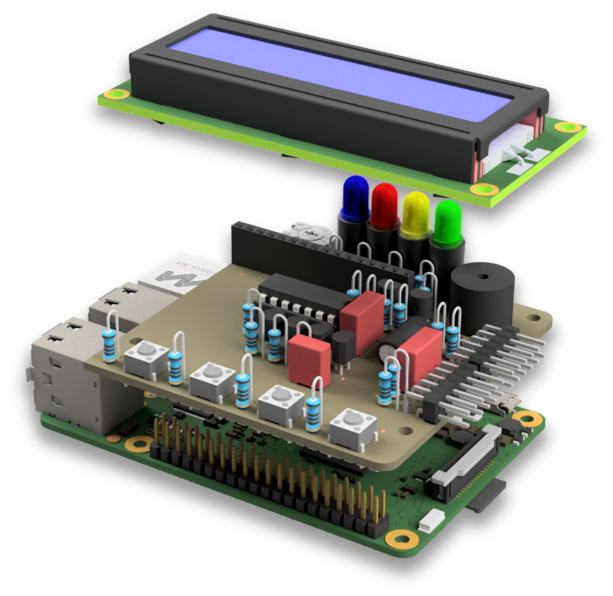
\includegraphics[scale=0.5]{abbildungen/hardwareentwurf.png}
      \caption{Hardware Grundaufbau für einen Sensorknoten (ohne Sensoren)}
 \end{figure}


\subsection{Mikrocontroller}

Als Mikrocontroller kommt ein Atmel ATTiny84 zum Einsatz. Auf diesem wurden die generischen Funktionen wie die ADC-Konversation, digitales Schalten und Lesen der Spannungspegel, sowie PWM-Funktionalitäten implementiert. Viele der Funktionalitäten lassen sich ebenfalls parametrisieren, wie die Referenzspannung der ADC-Wandlung, konfigurierbare Pullup-Widerstände beim Lesen der digitalen Eingänge uvm. Dies erlaubt eine generische Ansteuerung der Pins über den PI und erhöht somit die Flexibilität, da die Pins des Mikrocontrollers nicht mehr fest an bestimmte Aufgaben oder Funktionalitäten gebunden sind. 

 Alle Funktionen basieren auf dem Prinzip 0-N Eingabe-Parameter, Verarbeitung und Rückgabe von 0-N Ergebnissen. Anhand dieses Aufbaus wurde ein I²C Protokoll entworfen, welches einen Remote-Procedure Call durch den I²C Master erlaubt. Der Funktionsaufruf wird dabei gestartet, sobald der Master die benötigten Parameter übertragen hat und anschließend einen Restart (RST) an den Slave sendet. Sollte der Funktionsaufruf zum Zeitpunkt der Rückübertragung nicht vollständig beendet sein, wird die sogenannte „Clock-Hold“ Sonderfunktionalität des I²C Protokolls genutzt, welche es dem Client ermöglicht, die Übertragung zu pausieren. Nach Abschluss werden anschließend die Resultate an den Master zurückgesendet. Jedes übertrage Byte wird von dem empfangenden Teilnehmer bestätigt, andernfalls wird die Übertragung abgebrochen. Die letzten beiden Bytes entsprechen einem Status-Code, welcher über die erfolgreiche Ausführung der Prozedur bzw. dem ggf. entstandenen Fehler informiert, sowie eine Checksumme, welche eine Erkennung von Übertragungsfehler ermöglicht.

 Eine erstellte Python-Bibliothek implementiert die korrespondierenden RPC-Funktionsaufrufe auf dem Raspberry-Pi und prüft die Datenübertragung/Fehlercodes. Alle RPC-Aufrufe sind mit Unit-Tests abgedeckt, welche zusätzlich ebenfalls einen Hardware-Check durchführen. Hierfür müssen in 2er Gruppen eingeteilt Pins mittels Jumperkabeln verbunden werden, welche sich durch den entsprechenden Unit-Test gegenseitig auf Funktionalität testen. 

 \begin{figure}[h!]
      \centering
      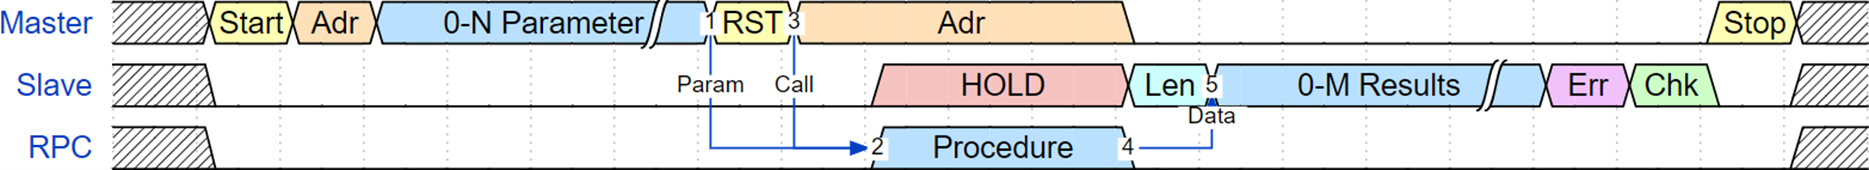
\includegraphics[scale=0.55]{abbildungen/kommunikationsProtokoll.png}
      \caption{Kommunikationsablauf zwischen Raspberry Pi und Mikrocontroller über I²C}
 \end{figure}